\documentclass{article}
% Author: Gianluigi Filippelli
% Based on calendar created by Till Tantau
\usepackage[a3paper]{geometry}
%
\usepackage{tikz}
\usetikzlibrary{calendar,folding}
%
\usepackage{xcolor}
\usepackage{ifthen}
%
\definecolor{space}{HTML}{1F2C4E}
\definecolor{earth}{HTML}{0089FA}
\definecolor{title}{HTML}{FBA706}
\definecolor{moon}{HTML}{AFAFAF}
\definecolor{spacetime}{HTML}{0CF508}
\definecolor{star}{HTML}{45457D}
\definecolor{mars}{HTML}{DC7B4E}
%
\usepackage{fontspec}
\setmainfont{Montserrat}
%
\title{Calendar 2022}
\begin{document}
	\pagestyle{empty}
	\tikzset{
		partial ellipse/.style args = {#1:#2:#3}{insert path={+ (#1:#3) arc (#1:#2:#3)}},
	}
	\begin{tikzpicture}[transform shape,
	every calendar/.style={
		at={(-8ex,4ex)},
		week list,
		month label above centered, 
		month text=\bfseries\textcolor{space}{\%mt} \%y0,
		if={(Sunday) [star]}
	}]
	%
		\begin{scope}
			\draw [black,ultra thick,fill=title] (0,7.5) rectangle (19,10.5);
			\node at (9.5,9.3) {\textcolor{black}{\fontsize{40}{41}\selectfont Calendar 2022}};
		\end{scope}
		\begin{scope}[shift={(-1,3.5)}]
			\draw [ultra thick, fill=earth!50!white] (-2.2,1.2) rectangle (2.5,-2.4);
			\calendar [dates=2022-01-01 to 2022-01-last];
		\end{scope}
		%
		\begin{scope}[scale=0.7]
			\draw [fill=space,ultra thick] (3.8,8) rectangle (30,1);
			%
			\foreach \c in {1,3,...,7}
			{
				\draw [fill=moon] (2.7 + \c*3.5,5) circle (1.5cm);
			}
			\draw [fill=black, opacity=0.5] (2.7 + 3.5,5) circle (1.5cm);
			\draw [fill=black, opacity=0.5] (2.7 + 3*3.5,5) [partial ellipse=90:270:1.5 and 1.5];
			\draw [fill=black, opacity=0.5] (2.7 + 7*3.5,5) [partial ellipse=-90:90:1.5 and 1.5];
			%
			\node at (2.7 + 3.5,7) {\textcolor{white}{\fontsize{17}{18}\selectfont New Moon}};
			\node at (2.7 + 3.5,3) {\textcolor{white}{\fontsize{17}{18}\selectfont January 2}};
			\node at (2.7 + 3.5,2) {\textcolor{white}{\fontsize{17}{18}\selectfont 19:33}};
			%
			\node at (2.7 + 3*3.5,7) {\textcolor{white}{\fontsize{17}{18}\selectfont First Quarter}};
			\node at (2.7 + 3*3.5,3) {\textcolor{white}{\fontsize{17}{18}\selectfont January 9}};
			\node at (2.7 + 3*3.5,2) {\textcolor{white}{\fontsize{17}{18}\selectfont 19:11}};
			%
			\node at (2.7 + 5*3.5,7) {\textcolor{white}{\fontsize{17}{18}\selectfont Full Moon}};
			\node at (2.7 + 5*3.5,3) {\textcolor{white}{\fontsize{17}{18}\selectfont January 18}};
			\node at (2.7 + 5*3.5,2) {\textcolor{white}{\fontsize{17}{18}\selectfont 00:48}};
			%
			\node at (2.7 + 7*3.5,7) {\textcolor{white}{\fontsize{17}{18}\selectfont Third Quarter}};
			\node at (2.7 + 7*3.5,3) {\textcolor{white}{\fontsize{17}{18}\selectfont January 25}};
			\node at (2.7 + 7*3.5,2) {\textcolor{white}{\fontsize{17}{18}\selectfont 14:41}};
		\end{scope}
		%
		\begin{scope}[shift={(-1,-3)}]
			\draw [ultra thick, fill=earth!50!white] (-2.2,1.2) rectangle (2.5,-2.4);
			\calendar [dates=2022-02-01 to 2022-02-last];
		\end{scope}
		%
		\begin{scope}[scale=0.7,shift={(0,-10)}]
			\draw [fill=space,ultra thick] (3.8,8) rectangle (30,1);
			%
			\foreach \c in {1,3,...,7}
			{
				\draw [fill=moon] (2.7 + \c*3.5,5) circle (1.5cm);
			}
			\draw [fill=black, opacity=0.5] (2.7 + 3.5,5) circle (1.5cm);
			\draw [fill=black, opacity=0.5] (2.7 + 3*3.5,5) [partial ellipse=90:270:1.5 and 1.5];
			\draw [fill=black, opacity=0.5] (2.7 + 7*3.5,5) [partial ellipse=-90:90:1.5 and 1.5];
			%
			\node at (2.7 + 3.5,7) {\textcolor{white}{\fontsize{17}{18}\selectfont New Moon}};
			\node at (2.7 + 3.5,3) {\textcolor{white}{\fontsize{17}{18}\selectfont February 1}};
			\node at (2.7 + 3.5,2) {\textcolor{white}{\fontsize{17}{18}\selectfont 06:46}};
			%
			\node at (2.7 + 3*3.5,7) {\textcolor{white}{\fontsize{17}{18}\selectfont First Quarter}};
			\node at (2.7 + 3*3.5,3) {\textcolor{white}{\fontsize{17}{18}\selectfont February 8}};
			\node at (2.7 + 3*3.5,2) {\textcolor{white}{\fontsize{17}{18}\selectfont 14:50}};
			%
			\node at (2.7 + 5*3.5,7) {\textcolor{white}{\fontsize{17}{18}\selectfont Full Moon}};
			\node at (2.7 + 5*3.5,3) {\textcolor{white}{\fontsize{17}{18}\selectfont February 16}};
			\node at (2.7 + 5*3.5,2) {\textcolor{white}{\fontsize{17}{18}\selectfont 17:56}};
			%
			\node at (2.7 + 7*3.5,7) {\textcolor{white}{\fontsize{17}{18}\selectfont Third Quarter}};
			\node at (2.7 + 7*3.5,3) {\textcolor{white}{\fontsize{17}{18}\selectfont February 23}};
			\node at (2.7 + 7*3.5,2) {\textcolor{white}{\fontsize{17}{18}\selectfont 23:32}};
		\end{scope}
		%
		\begin{scope}[shift={(-1,-9.5)}]
			\draw [ultra thick, fill=earth!50!white] (-2.2,1.2) rectangle (2.5,-2.4);
			\calendar [dates=2022-03-01 to 2022-03-last];
		\end{scope}
		%
		\begin{scope}[shift={(-1,-16)}]
			\draw [ultra thick, fill=earth!50!white] (-2.2,1.2) rectangle (2.5,-2.4);
			\calendar [dates=2022-04-01 to 2022-04-last];
		\end{scope}	
	\end{tikzpicture}
	%
	\newpage
	%
	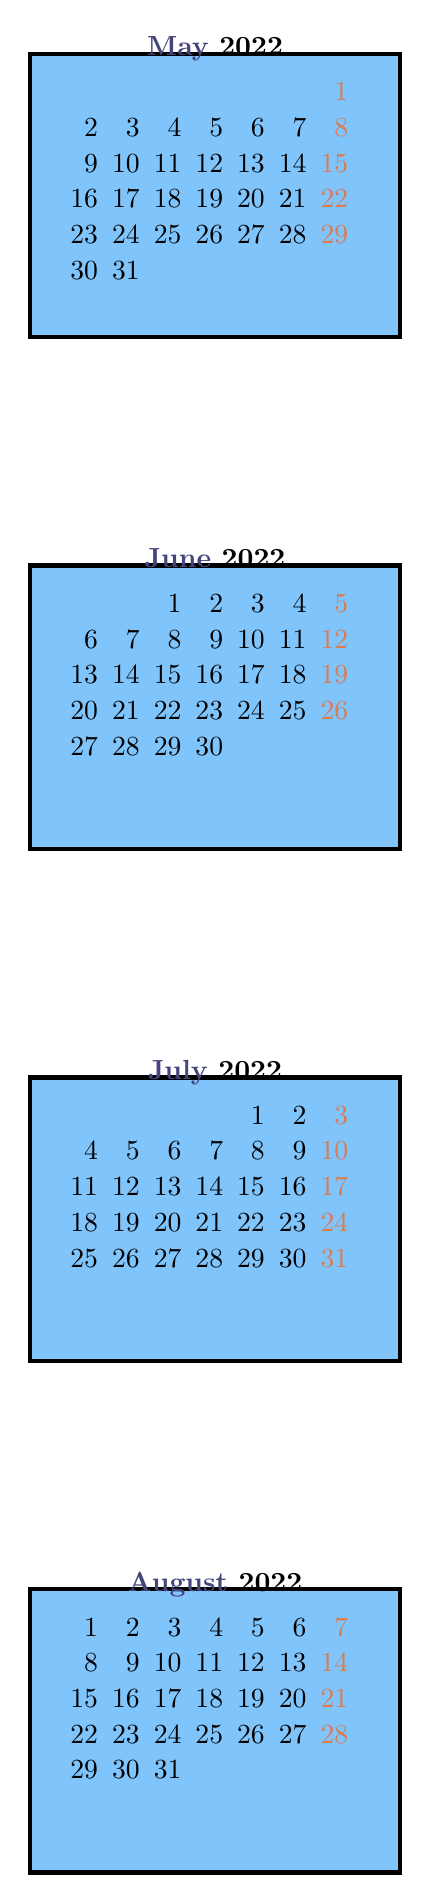
\begin{tikzpicture}[transform shape,
		every calendar/.style={
			at={(-8ex,4ex)},
			week list,
			month label above centered, 
			month text=\bfseries\textcolor{star}{\%mt} \%y0,
			if={(Sunday) [mars]}
		}]
		\begin{scope}[shift={(-1,3.5)}]
			\draw [ultra thick, fill=earth!50!white] (-2.2,1.2) rectangle (2.5,-2.4);
			\calendar [dates=2022-05-01 to 2022-05-last];
		\end{scope}
		%
		\begin{scope}[shift={(-1,-3)}]
			\draw [ultra thick, fill=earth!50!white] (-2.2,1.2) rectangle (2.5,-2.4);
			\calendar [dates=2022-06-01 to 2022-06-last];
		\end{scope}
		%
		\begin{scope}[shift={(-1,-9.5)}]
			\draw [ultra thick, fill=earth!50!white] (-2.2,1.2) rectangle (2.5,-2.4);
			\calendar [dates=2022-07-01 to 2022-07-last];
		\end{scope}
		%
		\begin{scope}[shift={(-1,-16)}]
			\draw [ultra thick, fill=earth!50!white] (-2.2,1.2) rectangle (2.5,-2.4);
			\calendar [dates=2022-08-01 to 2022-08-last];
		\end{scope}	
	\end{tikzpicture}
	%
	\newpage
	%
	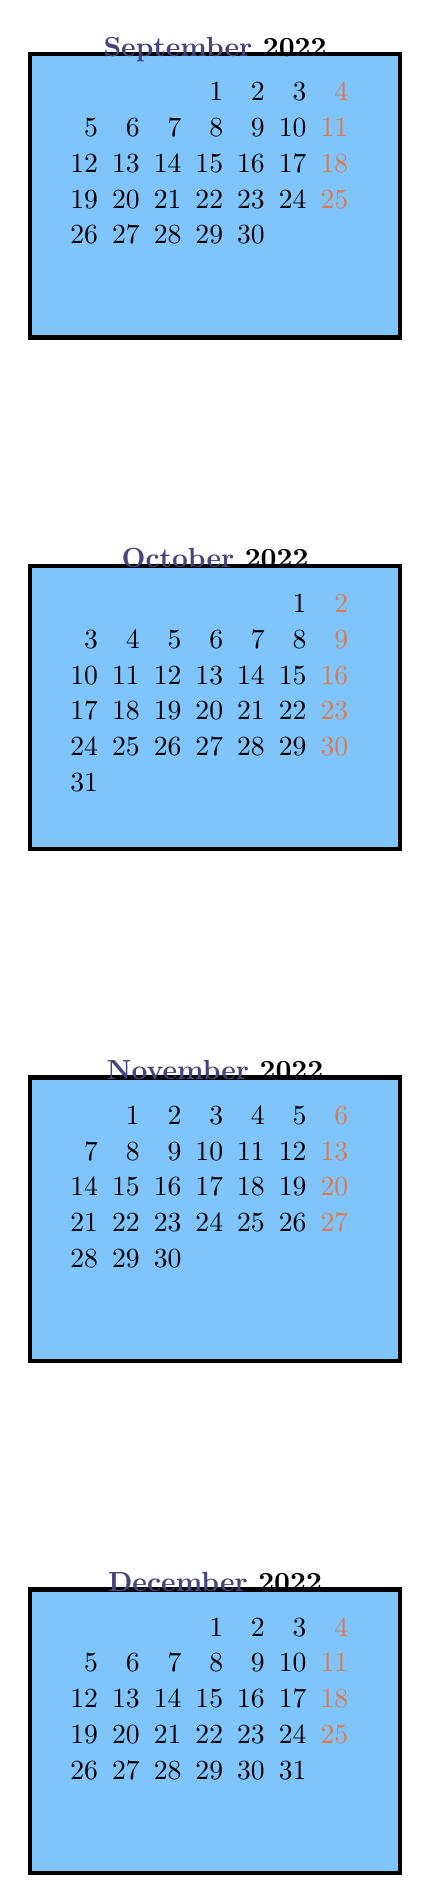
\begin{tikzpicture}[transform shape,
		every calendar/.style={
			at={(-8ex,4ex)},
			week list,
			month label above centered, 
			month text=\bfseries\textcolor{star}{\%mt} \%y0,
			if={(Sunday) [mars]}
		}]
		\begin{scope}[shift={(-1,3.5)}]
			\draw [ultra thick, fill=earth!50!white] (-2.2,1.2) rectangle (2.5,-2.4);
			\calendar [dates=2022-09-01 to 2022-09-last];
		\end{scope}
		%
		\begin{scope}[shift={(-1,-3)}]
			\draw [ultra thick, fill=earth!50!white] (-2.2,1.2) rectangle (2.5,-2.4);
			\calendar [dates=2022-10-01 to 2022-10-last];
		\end{scope}
		%
		\begin{scope}[shift={(-1,-9.5)}]
			\draw [ultra thick, fill=earth!50!white] (-2.2,1.2) rectangle (2.5,-2.4);
			\calendar [dates=2022-11-01 to 2022-11-last];
		\end{scope}
		%
		\begin{scope}[shift={(-1,-16)}]
			\draw [ultra thick, fill=earth!50!white] (-2.2,1.2) rectangle (2.5,-2.4);
			\calendar [dates=2022-12-01 to 2022-12-last];
		\end{scope}	
	\end{tikzpicture}
\end{document}

